\chapter{Appendix}

\section{Gantt Chart of Project Timeline}
\label{sec:appendix_a}

The Gantt chart in \cref{fig:gantt} is intended as a guideline; task bars are not drawn to an exact 1:1 temporal scale.

% \begin{figure}[h]
%     \centering
%     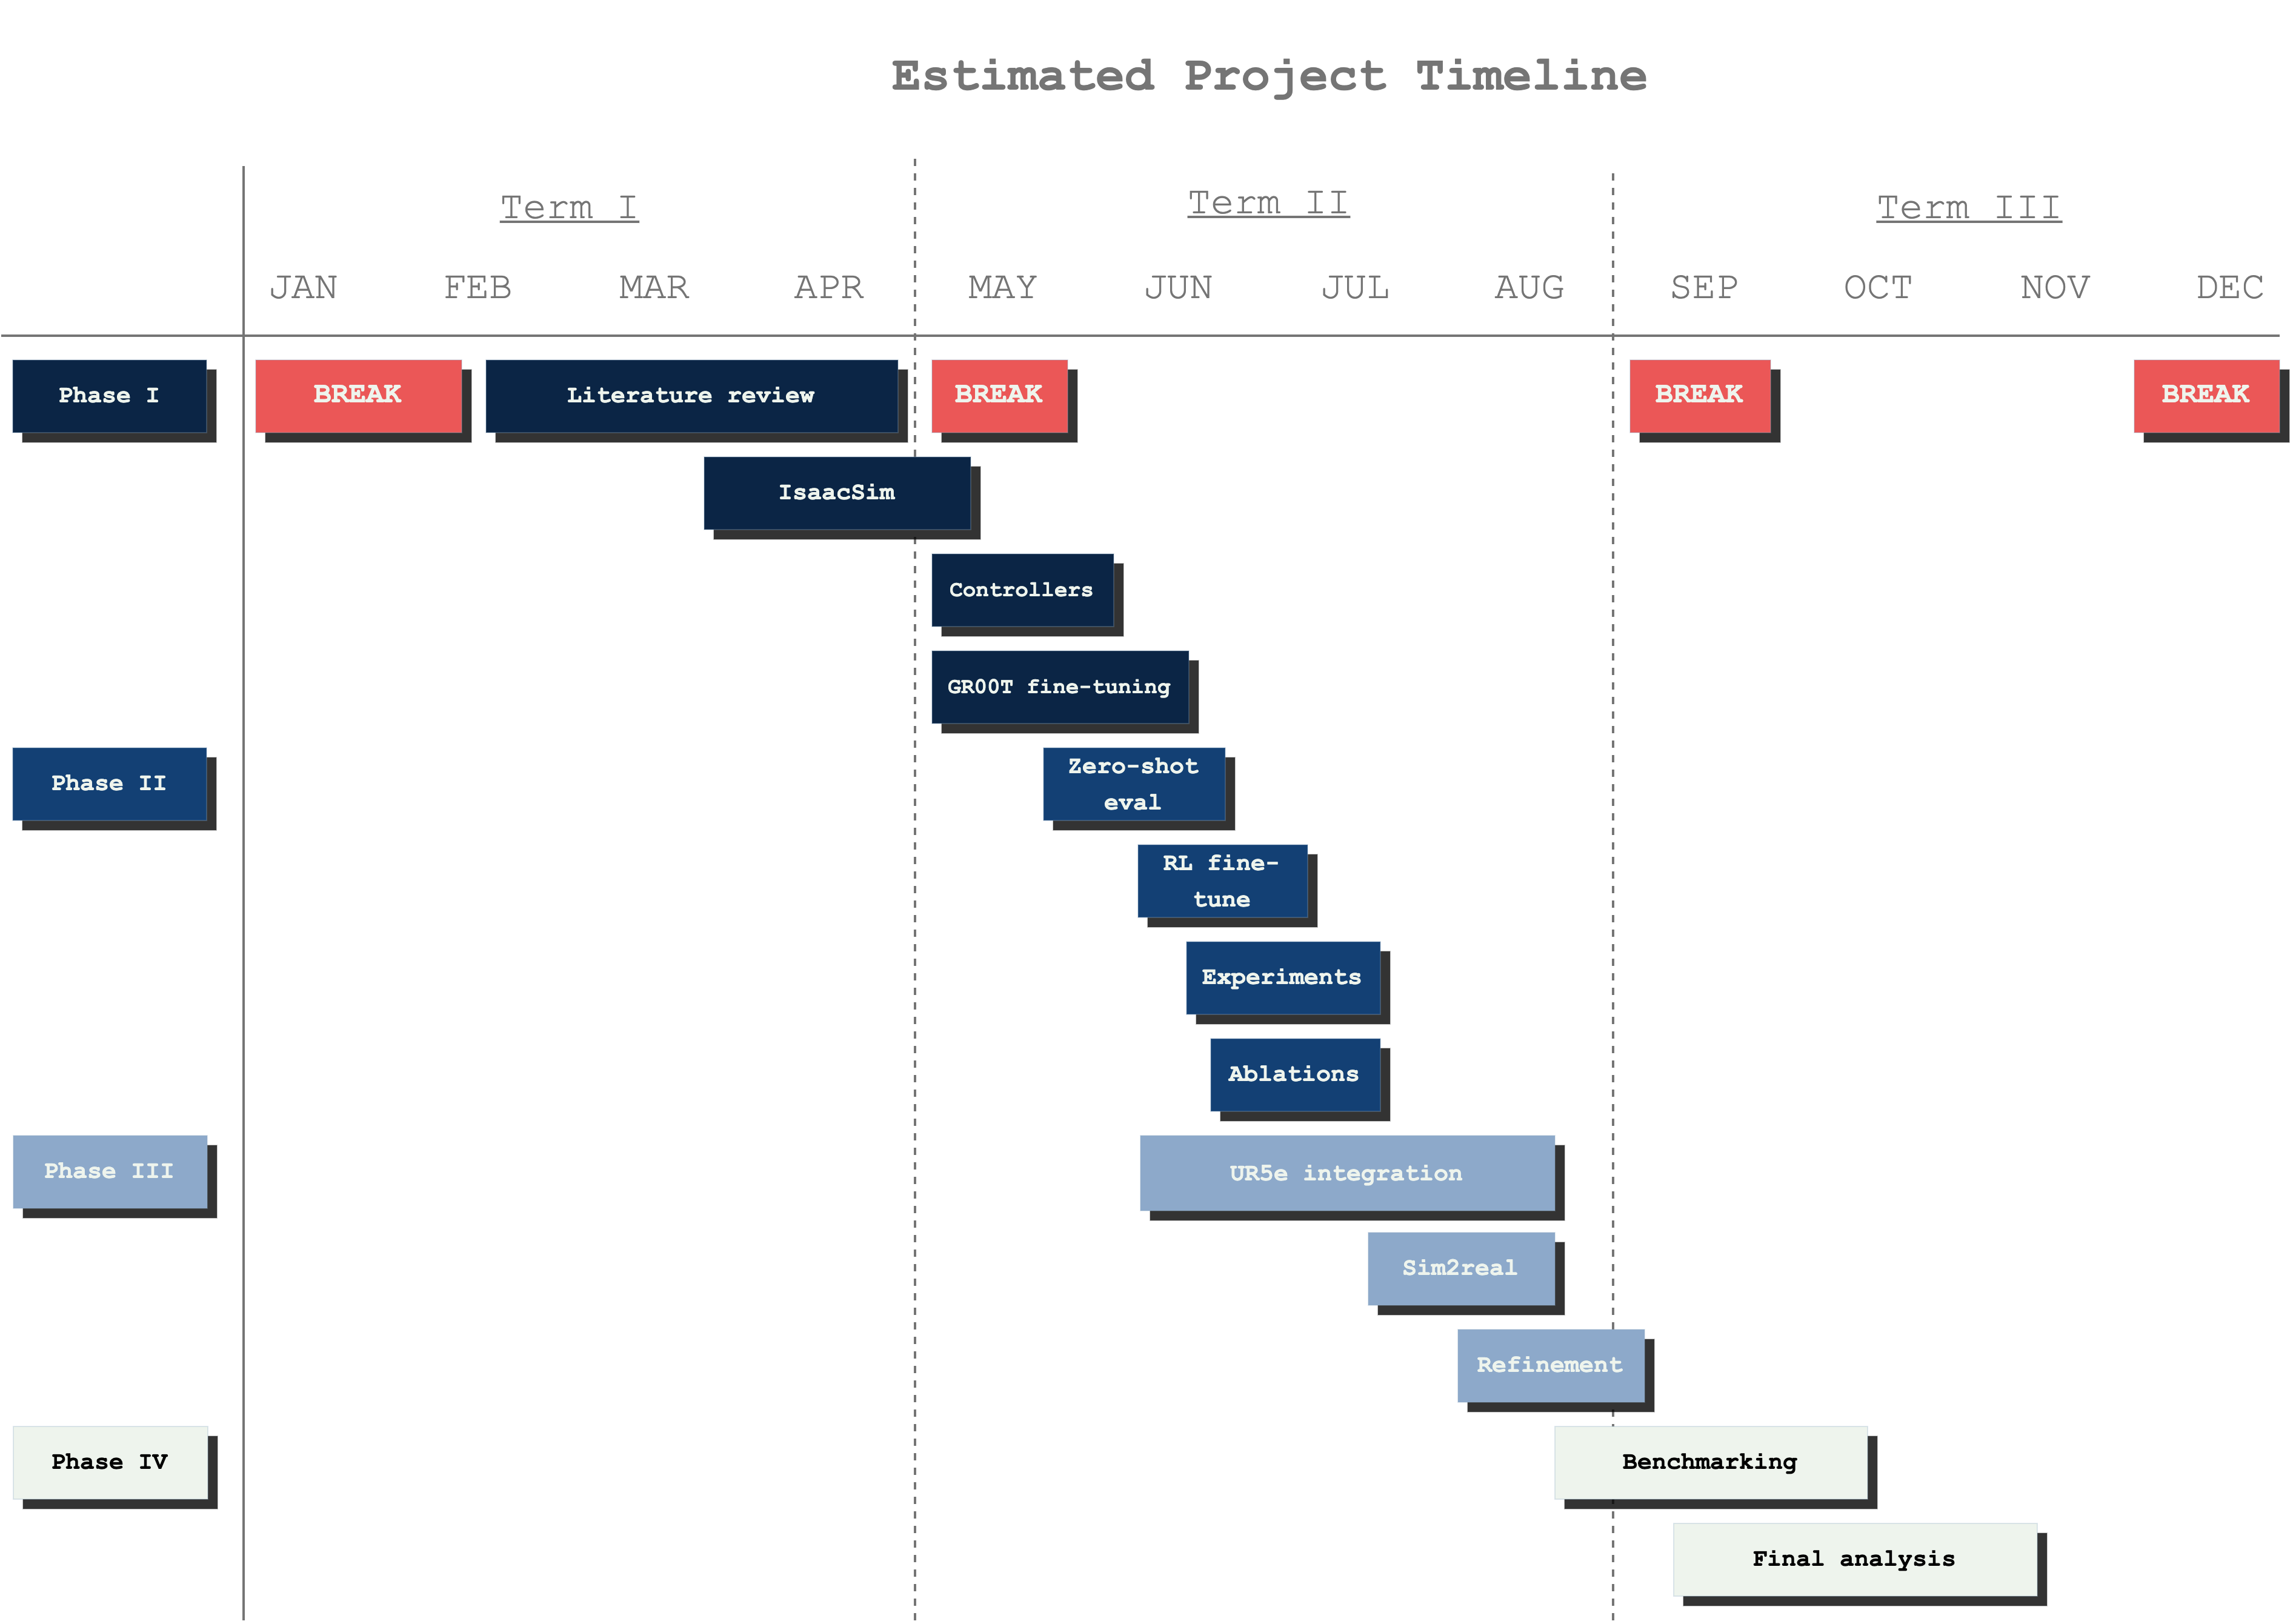
\includegraphics[width=\linewidth,height=0.75\textheight,keepaspectratio]{Figures/gantt.png}
%     \caption{Estimated project timeline broken down by academic term. The Gantt chart outlines four major phases of the project, beginning with simulation setup and literature review in Term 1, progressing through fine-tuning, evaluation, and integration in Term 2, and concluding with benchmarking and final analysis in Term 3. This timeline is a high-level guide and may be adjusted based on experimental findings and system performance.}
%     \label{fig:gantt}
% \end{figure}

\bigfigure[
    pos=H,
    opt={width=\linewidth,height=0.75\textheight,keepaspectratio},
    label={fig:gantt},
    shortcaption={Estimated project timeline by term, showing simulation setup, fine-tuning, evaluation, and final analysis phases.}
]
{gantt.png}
{Estimated project timeline broken down by academic term. The Gantt chart outlines four major phases of the project, beginning with simulation setup and literature review in Term 1, progressing through fine-tuning, evaluation, and integration in Term 2, and concluding with benchmarking and final analysis in Term 3. This timeline is a high-level guide and may be adjusted based on experimental findings and system performance.}

% \bigfigure[
%     pos=h,
%     opt={width=\linewidth},
%     \label{fig:gantt},
%     shortcaption={A short caption}
% ]
% {gantt.png}
% {Design process using a few \protect\acs{CFD} simulations (...) to be redone.}

\begin{widetablepages}
\begin{addmargin*}[0pt]{\fullmarginwidth}
\section{Full Discretized Task Progress Results}
\label{sec:appendix:results_monolith}

This appendix reports the per-trial \ac{DTP} scores $P_{\text{task}}$ for the frozen base policy, the three pure RL baselines (TD3, SAC, PPO), and their residual counterparts. Each method was evaluated on 20 physical rollouts per task under the 5--5--10 protocol.

The summary rows reproduce the values reported in \cref{tab:main_results_condensed}. Applying the metric definitions in \cref{sec:method:evaluation_metrics} to the printed trial rows gives different values for 60 of the 119 summary entries. For example, the 20 base-policy scores for \texttt{rubix-stack-v1} average 0.2500, while the reported mean is 0.2625. Reconciling these values requires the original rollout records.

\end{addmargin*}

\footnotesize
\begin{longtable}{@{\extracolsep{\fill}}l c *{7}{c} @{}}
    \caption[Full discretized task progress results]%
    {Full discretized task progress $P_{\text{task}}$ for all $7$ tasks and $20$ real-world rollouts per method. Columns report \ac{DTP} for the base policy, three pure RL baselines, and three residual RL adapters (\ac{TD3}, \ac{SAC}, \ac{PPO}) composed with the base policy. Trials are grouped into \ac{ID}, DP (dynamic perturbation), and \ac{OOD} conditions.}

    
    \label{tab:main_results} \\

    \toprule
    \multirow{2}{*}{\textbf{Block}} &
    \multirow{2}{*}{\textbf{Trial}} &
    % \multirow{2}{*}{\textbf{Base policy}} &
    \multirow{2}{*}{\shortstack[c]{\textbf{Base}\\\textbf{policy}}} &
    \multicolumn{3}{c}{\textbf{RL only}} &
    \multicolumn{3}{c}{\textbf{Residual}} \\
    \cmidrule(lr){4-6}\cmidrule(lr){7-9}
      &   &   & \textbf{TD3} & \textbf{SAC} & \textbf{PPO}
              & \textbf{TD3} & \textbf{SAC} & \textbf{PPO} \\
    \midrule
    \endfirsthead

    \multicolumn{9}{@{}l}{\textit{Table~\thetable\ (continued). Trials 1--5 are ID, 6--10 are DP, and 11--20 are OOD.}} \\
    \toprule
    \multirow{2}{*}{\textbf{Block}} &
    \multirow{2}{*}{\textbf{Trial}} &
    % \multirow{2}{*}{\textbf{Base policy}} &
    \multirow{2}{*}{\shortstack[c]{\textbf{Base}\\\textbf{policy}}} &
    \multicolumn{3}{c}{\textbf{RL only}} &
    \multicolumn{3}{c}{\textbf{Residual}} \\
    \cmidrule(lr){4-6}\cmidrule(lr){7-9}
      &   &   & \textbf{TD3} & \textbf{SAC} & \textbf{PPO}
              & \textbf{TD3} & \textbf{SAC} & \textbf{PPO} \\
    \midrule
    \endhead

    \midrule \multicolumn{9}{r@{}}{\textit{(continued on next page)}} \\
    \endfoot

    \bottomrule
    \endlastfoot

    %%%%%%%%%%%%%%%%%%%%%%%%%%%%%%%%%%%%%%%%%%%%%%%%%%%%%%%%%%%%%%
    % Task 1
    %%%%%%%%%%%%%%%%%%%%%%%%%%%%%%%%%%%%%%%%%%%%%%%%%%%%%%%%%%%%%%
    \multicolumn{9}{@{}l}{Task 1: \texttt{rubix-stack-v1}} \\*
    % --- In Distribution (1-5) ---
    \midrule
    \acs{ID}
      &  1 & 0.2500 & 0.2500 & 0.2500 & 0.2500 & 0.7500 & 0.5000 & 0.7500 \\
      &  2 & 0.5000 & 0.5000 & 0.5000 & 0.2500 & 0.7500 & 0.5000 & 0.7500 \\
      &  3 & 0.2500 & 0.2500 & 0.2500 & 0.2500 & 0.7500 & 0.5000 & 0.7500 \\
      &  4 & 0.5000 & 0.2500 & 0.2500 & 0.2500 & 0.7500 & 0.5000 & 0.7500 \\
      &  5 & 0.2500 & 0.2500 & 0.2500 & 0.2500 & 0.7500 & 0.5000 & 0.7500 \\
    \midrule
    % --- Dynamic Perturbation (6-10) ---
    DP
      &  6 & 0.5000 & 0.5000 & 0.5000 & 0.2500 & 0.7500 & 0.5000 & 0.7500 \\
      &  7 & 0.2500 & 0.2500 & 0.2500 & 0.2500 & 0.7500 & 0.5000 & 0.7500 \\
      &  8 & 0.5000 & 0.2500 & 0.2500 & 0.2500 & 0.7500 & 0.5000 & 0.7500 \\
      &  9 & 0.2500 & 0.2500 & 0.2500 & 0.2500 & 0.7500 & 0.5000 & 0.7500 \\
      & 10 & 0.5000 & 0.5000 & 0.5000 & 0.2500 & 0.7500 & 0.5000 & 0.7500 \\
    \midrule
    % --- OOD (11-20) ---
    \acs{OOD}
      & 11 & 0.2500 & 0.2500 & 0.2500 & 0.2500 & 0.7500 & 0.5000 & 0.7500 \\
      & 12 & 0.0000 & 0.0000 & 0.2500 & 0.0000 & 0.5000 & 0.2500 & 0.5000 \\
      & 13 & 0.2500 & 0.2500 & 0.5000 & 0.2500 & 0.7500 & 0.5000 & 0.7500 \\
      & 14 & 0.0000 & 0.0000 & 0.2500 & 0.0000 & 0.5000 & 0.2500 & 0.5000 \\
      & 15 & 0.2500 & 0.2500 & 0.0000 & 0.2500 & 0.7500 & 0.5000 & 0.7500 \\
      & 16 & 0.0000 & 0.0000 & 0.2500 & 0.0000 & 0.5000 & 0.2500 & 0.5000 \\
      & 17 & 0.2500 & 0.2500 & 0.2500 & 0.2500 & 0.7500 & 0.5000 & 0.7500 \\
      & 18 & 0.0000 & 0.0000 & 0.2500 & 0.0000 & 0.5000 & 0.2500 & 0.5000 \\
      & 19 & 0.2500 & 0.2500 & 0.5000 & 0.2500 & 0.7500 & 0.5000 & 0.7500 \\
      & 20 & 0.0000 & 0.0000 & 0.2500 & 0.0000 & 0.5000 & 0.2500 & 0.5000 \\
    \midrule
    \addlinespace
    \multicolumn{2}{r}{Mean progress $MP$}             &
        0.2625 & 0.2375 & 0.2750 & 0.2125 & 0.6750 & 0.4375 & 0.6750 \\
    \multicolumn{2}{r}{Generalization $J_{\text{gen}}$} &
        0.1250 & 0.1250 & 0.2500 & 0.1250 & 0.6000 & 0.3750 & 0.6000 \\
    \multicolumn{2}{r}{Transfer gap $\Delta_{\text{gen}}$} &
        \multicolumn{1}{c}{--} &  % Base
        \multicolumn{1}{c}{--} &  % RL TD3
        \multicolumn{1}{c}{--} &  % RL SAC
        \multicolumn{1}{c}{--} &  % RL PPO
        \multicolumn{1}{c}{0.4750} & % Res TD3
        \multicolumn{1}{c}{0.2500} & % Res SAC
        \multicolumn{1}{c}{0.4750}   % Res PPO
        \\
    \addlinespace
    \midrule

    %%%%%%%%%%%%%%%%%%%%%%%%%%%%%%%%%%%%%%%%%%%%%%%%%%%%%%%%%%%%%%
    % Task 2
    %%%%%%%%%%%%%%%%%%%%%%%%%%%%%%%%%%%%%%%%%%%%%%%%%%%%%%%%%%%%%%
    \multicolumn{9}{@{}l}{Task 2: \texttt{bus-table-easy-v1}} \\*
    % --- In Distribution (1-5) ---
    \midrule
    \acs{ID}
      &  1 & 0.2500 & 0.0000 & 0.0000 & 0.0000 & 0.2500 & 0.2500 & 0.2500 \\
      &  2 & 0.5000 & 0.2500 & 0.2500 & 0.2500 & 0.5000 & 0.5000 & 0.5000 \\
      &  3 & 0.2500 & 0.0000 & 0.5000 & 0.0000 & 0.2500 & 0.2500 & 0.2500 \\
      &  4 & 0.5000 & 0.2500 & 0.2500 & 0.2500 & 0.5000 & 0.5000 & 0.5000 \\
      &  5 & 0.2500 & 0.0000 & 0.0000 & 0.0000 & 0.2500 & 0.2500 & 0.2500 \\
    \midrule
    % --- Dynamic Perturbation (6-10) ---
    DP
      &  6 & 0.5000 & 0.2500 & 0.2500 & 0.2500 & 0.5000 & 0.5000 & 0.5000 \\
      &  7 & 0.2500 & 0.0000 & 0.5000 & 0.0000 & 0.2500 & 0.2500 & 0.2500 \\
      &  8 & 0.5000 & 0.2500 & 0.2500 & 0.2500 & 0.5000 & 0.5000 & 0.5000 \\
      &  9 & 0.2500 & 0.0000 & 0.0000 & 0.0000 & 0.2500 & 0.2500 & 0.2500 \\
      & 10 & 0.5000 & 0.2500 & 0.2500 & 0.2500 & 0.5000 & 0.5000 & 0.5000 \\
    \midrule
    % --- OOD (11-20) ---
    \acs{OOD}
      & 11 & 0.2500 & 0.2500 & 0.2500 & 0.2500 & 0.5000 & 0.5000 & 0.5000 \\
      & 12 & 0.7500 & 0.7500 & 0.7500 & 0.7500 & 1.0000 & 0.7500 & 1.0000 \\
      & 13 & 0.5000 & 0.5000 & 0.5000 & 0.5000 & 0.7500 & 0.7500 & 0.7500 \\
      & 14 & 0.7500 & 0.7500 & 1.0000 & 0.7500 & 1.0000 & 1.0000 & 1.0000 \\
      & 15 & 0.5000 & 0.5000 & 0.5000 & 0.5000 & 0.7500 & 0.7500 & 0.7500 \\
      & 16 & 0.7500 & 0.7500 & 0.7500 & 0.5000 & 1.0000 & 1.0000 & 1.0000 \\
      & 17 & 0.5000 & 0.5000 & 0.5000 & 0.5000 & 0.7500 & 0.7500 & 0.7500 \\
      & 18 & 0.7500 & 0.7500 & 0.7500 & 0.7500 & 1.0000 & 0.7500 & 1.0000 \\
      & 19 & 0.5000 & 0.5000 & 0.5000 & 0.5000 & 0.7500 & 0.7500 & 0.7500 \\
      & 20 & 0.7500 & 0.7500 & 1.0000 & 0.7500 & 1.0000 & 1.0000 & 1.0000 \\
    \midrule
    \addlinespace
    \multicolumn{2}{r}{Mean progress $MP$}             &
        0.5000 & 0.3625 & 0.4500 & 0.3375 & 0.6750 & 0.6000 & 0.6750 \\
    \multicolumn{2}{r}{Generalization $J_{\text{gen}}$} &
        0.6250 & 0.6250 & 0.6750 & 0.5750 & 0.8750 & 0.8000 & 0.8750 \\
    \multicolumn{2}{r}{Transfer gap $\Delta_{\text{gen}}$} &
        \multicolumn{1}{c}{--} &  % Base
        \multicolumn{1}{c}{--} &  % RL TD3
        \multicolumn{1}{c}{--} &  % RL SAC
        \multicolumn{1}{c}{--} &  % RL PPO
        \multicolumn{1}{c}{0.2500} & % Res TD3
        \multicolumn{1}{c}{0.1750} & % Res SAC
        \multicolumn{1}{c}{0.2500}   % Res PPO
        \\
    \addlinespace
    \midrule

    %%%%%%%%%%%%%%%%%%%%%%%%%%%%%%%%%%%%%%%%%%%%%%%%%%%%%%%%%%%%%%
    % Task 3
    %%%%%%%%%%%%%%%%%%%%%%%%%%%%%%%%%%%%%%%%%%%%%%%%%%%%%%%%%%%%%%
    \multicolumn{9}{@{}l}{Task 3: \texttt{bus-table-medium-v1}} \\*
    % --- In Distribution (1-5) ---
    \midrule
    \acs{ID}
      &  1 & 0.2500 & 0.0000 & 0.2500 & 0.0000 & 0.2500 & 0.2500 & 0.2500 \\
      &  2 & 0.5000 & 0.2500 & 0.2500 & 0.2500 & 0.5000 & 0.5000 & 0.5000 \\
      &  3 & 0.2500 & 0.0000 & 0.0000 & 0.0000 & 0.2500 & 0.2500 & 0.2500 \\
      &  4 & 0.5000 & 0.2500 & 0.2500 & 0.2500 & 0.5000 & 0.7500 & 0.5000 \\
      &  5 & 0.2500 & 0.0000 & 0.2500 & 0.0000 & 0.2500 & 0.2500 & 0.2500 \\
    \midrule
    % --- Dynamic Perturbation (6-10) ---
    DP
      &  6 & 0.5000 & 0.2500 & 0.2500 & 0.2500 & 0.5000 & 0.5000 & 0.5000 \\
      &  7 & 0.2500 & 0.0000 & 0.0000 & 0.0000 & 0.2500 & 0.2500 & 0.2500 \\
      &  8 & 0.5000 & 0.2500 & 0.2500 & 0.2500 & 0.5000 & 0.7500 & 0.5000 \\
      &  9 & 0.2500 & 0.0000 & 0.2500 & 0.0000 & 0.2500 & 0.2500 & 0.2500 \\
      & 10 & 0.5000 & 0.2500 & 0.2500 & 0.2500 & 0.5000 & 0.5000 & 0.5000 \\
    \midrule
    % --- OOD (11-20) ---
    \acs{OOD}
      & 11 & 0.2500 & 0.0000 & 0.0000 & 0.0000 & 0.5000 & 0.2500 & 0.5000 \\
      & 12 & 0.2500 & 0.2500 & 0.2500 & 0.2500 & 0.7500 & 0.7500 & 0.7500 \\
      & 13 & 0.0000 & 0.0000 & 0.2500 & 0.0000 & 0.5000 & 0.5000 & 0.5000 \\
      & 14 & 0.2500 & 0.2500 & 0.5000 & 0.2500 & 0.7500 & 0.7500 & 0.7500 \\
      & 15 & 0.0000 & 0.0000 & 0.2500 & 0.0000 & 0.5000 & 0.5000 & 0.5000 \\
      & 16 & 0.2500 & 0.2500 & 0.0000 & 0.0000 & 0.5000 & 0.5000 & 0.5000 \\
      & 17 & 0.0000 & 0.0000 & 0.2500 & 0.2500 & 0.5000 & 0.5000 & 0.5000 \\
      & 18 & 0.2500 & 0.2500 & 0.2500 & 0.2500 & 0.7500 & 0.7500 & 0.7500 \\
      & 19 & 0.0000 & 0.0000 & 0.2500 & 0.0000 & 0.5000 & 0.5000 & 0.5000 \\
      & 20 & 0.2500 & 0.2500 & 0.5000 & 0.2500 & 0.7500 & 0.7500 & 0.7500 \\
    \midrule
    \addlinespace
    \multicolumn{2}{r}{Mean progress $MP$}             &
        0.3125 & 0.1875 & 0.3125 & 0.1750 & 0.5500 & 0.5375 & 0.5250 \\
    \multicolumn{2}{r}{Generalization $J_{\text{gen}}$} &
        0.2500 & 0.1500 & 0.2750 & 0.1250 & 0.6000 & 0.6000 & 0.6000 \\
    \multicolumn{2}{r}{Transfer gap $\Delta_{\text{gen}}$} &
        \multicolumn{1}{c}{--} &  % Base
        \multicolumn{1}{c}{--} &  % RL TD3
        \multicolumn{1}{c}{--} &  % RL SAC
        \multicolumn{1}{c}{--} &  % RL PPO
        \multicolumn{1}{c}{0.3500} & % Res TD3
        \multicolumn{1}{c}{0.4500} & % Res SAC
        \multicolumn{1}{c}{0.3500}   % Res PPO
        \\
    \addlinespace
    \midrule

    %%%%%%%%%%%%%%%%%%%%%%%%%%%%%%%%%%%%%%%%%%%%%%%%%%%%%%%%%%%%%%
    % Task 4
    %%%%%%%%%%%%%%%%%%%%%%%%%%%%%%%%%%%%%%%%%%%%%%%%%%%%%%%%%%%%%%
    \multicolumn{9}{@{}l}{Task 4: \texttt{bus-table-hard-v1}} \\*
    % --- In Distribution (1-5) ---
    \midrule
    \acs{ID}
      &  1 & 0.0000 & 0.0000 & 0.0000 & 0.0000 & 0.2500 & 0.2500 & 0.2500 \\
      &  2 & 0.2500 & 0.2500 & 0.2500 & 0.0000 & 0.5000 & 0.5000 & 0.5000 \\
      &  3 & 0.0000 & 0.0000 & 0.0000 & 0.0000 & 0.2500 & 0.2500 & 0.2500 \\
      &  4 & 0.2500 & 0.0000 & 0.2500 & 0.0000 & 0.5000 & 0.5000 & 0.5000 \\
      &  5 & 0.0000 & 0.0000 & 0.0000 & 0.0000 & 0.2500 & 0.2500 & 0.2500 \\
    \midrule
    % --- Dynamic Perturbation (6-10) ---
    DP
      &  6 & 0.2500 & 0.2500 & 0.2500 & 0.0000 & 0.5000 & 0.5000 & 0.5000 \\
      &  7 & 0.0000 & 0.0000 & 0.0000 & 0.0000 & 0.2500 & 0.2500 & 0.2500 \\
      &  8 & 0.2500 & 0.0000 & 0.2500 & 0.0000 & 0.5000 & 0.5000 & 0.5000 \\
      &  9 & 0.0000 & 0.0000 & 0.0000 & 0.0000 & 0.2500 & 0.2500 & 0.2500 \\
      & 10 & 0.2500 & 0.2500 & 0.2500 & 0.0000 & 0.5000 & 0.5000 & 0.5000 \\
    \midrule
    % --- OOD (11-20) ---
    \acs{OOD}
      & 11 & 0.0000 & 0.0000 & 0.2500 & 0.0000 & 0.5000 & 0.5000 & 0.5000 \\
      & 12 & 0.0000 & 0.2500 & 0.0000 & 0.2500 & 0.5000 & 0.5000 & 0.5000 \\
      & 13 & 0.2500 & 0.0000 & 0.2500 & 0.0000 & 0.7500 & 0.7500 & 0.7500 \\
      & 14 & 0.0000 & 0.2500 & 0.0000 & 0.2500 & 0.5000 & 0.7500 & 0.5000 \\
      & 15 & 0.2500 & 0.0000 & 0.2500 & 0.0000 & 0.7500 & 0.7500 & 0.7500 \\
      & 16 & 0.0000 & 0.2500 & 0.0000 & 0.2500 & 0.5000 & 0.5000 & 0.5000 \\
      & 17 & 0.2500 & 0.0000 & 0.2500 & 0.0000 & 0.7500 & 0.7500 & 0.7500 \\
      & 18 & 0.0000 & 0.2500 & 0.0000 & 0.2500 & 0.5000 & 0.7500 & 0.5000 \\
      & 19 & 0.2500 & 0.0000 & 0.2500 & 0.0000 & 0.7500 & 0.7500 & 0.7500 \\
      & 20 & 0.0000 & 0.2500 & 0.0000 & 0.2500 & 0.5000 & 0.5000 & 0.5000 \\
    \midrule
    \addlinespace
    \multicolumn{2}{r}{Mean progress $MP$}             &
        0.2188 & 0.1562 & 0.2188 & 0.0625 & 0.5625 & 0.5312 & 0.5312 \\
    \multicolumn{2}{r}{Generalization $J_{\text{gen}}$} &
        0.1250 & 0.1250 & 0.2250 & 0.1250 & 0.6000 & 0.6250 & 0.6000 \\
    \multicolumn{2}{r}{Transfer gap $\Delta_{\text{gen}}$} &
        \multicolumn{1}{c}{--} &  % Base
        \multicolumn{1}{c}{--} &  % RL TD3
        \multicolumn{1}{c}{--} &  % RL SAC
        \multicolumn{1}{c}{--} &  % RL PPO
        \multicolumn{1}{c}{0.4750} & % Res TD3
        \multicolumn{1}{c}{0.5000} & % Res SAC
        \multicolumn{1}{c}{0.4750}   % Res PPO
        \\
    \addlinespace
    \midrule

    %%%%%%%%%%%%%%%%%%%%%%%%%%%%%%%%%%%%%%%%%%%%%%%%%%%%%%%%%%%%%%
    % Task 5
    %%%%%%%%%%%%%%%%%%%%%%%%%%%%%%%%%%%%%%%%%%%%%%%%%%%%%%%%%%%%%%
    \multicolumn{9}{@{}l}{Task 5: \texttt{close-bottle-lid-v1}} \\*
    % --- In Distribution (1-5) ---
    \midrule
    \acs{ID}
      &  1 & 0.7500 & 0.2500 & 0.2500 & 0.2500 & 0.5000 & 0.5000 & 0.7500 \\
      &  2 & 0.7500 & 0.2500 & 0.5000 & 0.2500 & 0.7500 & 0.7500 & 0.7500 \\
      &  3 & 0.5000 & 0.2500 & 0.2500 & 0.2500 & 0.5000 & 0.5000 & 0.7500 \\
      &  4 & 0.7500 & 0.2500 & 0.5000 & 0.2500 & 0.7500 & 0.7500 & 0.7500 \\
      &  5 & 0.7500 & 0.2500 & 0.2500 & 0.2500 & 0.5000 & 0.5000 & 0.7500 \\
    \midrule
    % --- Dynamic Perturbation (6-10) ---
    DP
      &  6 & 0.7500 & 0.2500 & 0.5000 & 0.2500 & 0.7500 & 0.7500 & 0.7500 \\
      &  7 & 0.5000 & 0.2500 & 0.2500 & 0.2500 & 0.5000 & 0.5000 & 0.7500 \\
      &  8 & 0.7500 & 0.2500 & 0.5000 & 0.2500 & 0.7500 & 0.7500 & 0.7500 \\
      &  9 & 0.7500 & 0.2500 & 0.2500 & 0.2500 & 0.5000 & 0.5000 & 0.7500 \\
      & 10 & 0.5000 & 0.2500 & 0.5000 & 0.2500 & 0.7500 & 0.7500 & 0.7500 \\
    \midrule
    % --- OOD (11-20) ---
    \acs{OOD}
      & 11 & 0.5000 & 0.2500 & 0.2500 & 0.2500 & 0.5000 & 0.5000 & 0.7500 \\
      & 12 & 0.5000 & 0.5000 & 0.5000 & 0.5000 & 0.7500 & 0.7500 & 0.7500 \\
      & 13 & 0.2500 & 0.2500 & 0.5000 & 0.2500 & 0.5000 & 0.7500 & 0.7500 \\
      & 14 & 0.5000 & 0.5000 & 0.5000 & 0.5000 & 0.7500 & 0.7500 & 0.7500 \\
      & 15 & 0.2500 & 0.2500 & 0.2500 & 0.2500 & 0.5000 & 0.5000 & 0.7500 \\
      & 16 & 0.5000 & 0.5000 & 0.5000 & 0.5000 & 0.7500 & 0.7500 & 0.7500 \\
      & 17 & 0.2500 & 0.2500 & 0.5000 & 0.2500 & 0.5000 & 0.7500 & 0.7500 \\
      & 18 & 0.5000 & 0.5000 & 0.5000 & 0.5000 & 0.7500 & 0.7500 & 0.7500 \\
      & 19 & 0.2500 & 0.2500 & 0.2500 & 0.2500 & 0.5000 & 0.5000 & 0.7500 \\
      & 20 & 0.5000 & 0.5000 & 0.5000 & 0.5000 & 0.7500 & 0.7500 & 0.7500 \\
    \midrule
    \addlinespace
    \multicolumn{2}{r}{Mean progress $MP$}             &
        0.5750 & 0.3125 & 0.4375 & 0.3125 & 0.6250 & 0.6500 & 0.7500 \\
    \multicolumn{2}{r}{Generalization $J_{\text{gen}}$} &
        0.4000 & 0.3750 & 0.4250 & 0.3750 & 0.6500 & 0.7000 & 0.7500 \\
    \multicolumn{2}{r}{Transfer gap $\Delta_{\text{gen}}$} &
        \multicolumn{1}{c}{--} &  % Base
        \multicolumn{1}{c}{--} &  % RL TD3
        \multicolumn{1}{c}{--} &  % RL SAC
        \multicolumn{1}{c}{--} &  % RL PPO
        \multicolumn{1}{c}{0.2500} & % Res TD3
        \multicolumn{1}{c}{0.3000} & % Res SAC
        \multicolumn{1}{c}{0.3500}   % Res PPO
        \\
    \addlinespace
    \midrule

    %%%%%%%%%%%%%%%%%%%%%%%%%%%%%%%%%%%%%%%%%%%%%%%%%%%%%%%%%%%%%%
    % Task 6
    %%%%%%%%%%%%%%%%%%%%%%%%%%%%%%%%%%%%%%%%%%%%%%%%%%%%%%%%%%%%%%
    \multicolumn{9}{@{}l}{Task 6: \texttt{erase-whiteboard-v1}} \\*
    % --- In Distribution (1-5) ---
    \midrule
    \acs{ID}
      &  1 & 1.0000 & 0.7500 & 0.7500 & 0.5000 & 1.0000 & 1.0000 & 1.0000 \\
      &  2 & 0.7500 & 0.7500 & 0.7500 & 0.7500 & 1.0000 & 1.0000 & 0.7500 \\
      &  3 & 1.0000 & 0.7500 & 1.0000 & 0.7500 & 1.0000 & 1.0000 & 1.0000 \\
      &  4 & 0.7500 & 0.7500 & 0.7500 & 0.7500 & 1.0000 & 1.0000 & 0.7500 \\
      &  5 & 1.0000 & 0.7500 & 1.0000 & 0.7500 & 1.0000 & 1.0000 & 1.0000 \\
    \midrule
    % --- Dynamic Perturbation (6-10) ---
    DP
      &  6 & 0.7500 & 0.7500 & 0.7500 & 0.7500 & 1.0000 & 1.0000 & 0.7500 \\
      &  7 & 1.0000 & 0.7500 & 1.0000 & 0.7500 & 1.0000 & 1.0000 & 1.0000 \\
      &  8 & 0.7500 & 0.7500 & 0.7500 & 0.7500 & 1.0000 & 1.0000 & 0.7500 \\
      &  9 & 1.0000 & 0.7500 & 1.0000 & 0.7500 & 1.0000 & 1.0000 & 1.0000 \\
      & 10 & 0.7500 & 0.7500 & 0.7500 & 0.7500 & 1.0000 & 1.0000 & 0.7500 \\
    \midrule
    % --- OOD (11-20) ---
    \acs{OOD}
      & 11 & 0.7500 & 0.5000 & 0.7500 & 0.5000 & 1.0000 & 1.0000 & 1.0000 \\
      & 12 & 0.7500 & 0.7500 & 0.7500 & 0.7500 & 0.7500 & 1.0000 & 0.7500 \\
      & 13 & 0.5000 & 0.5000 & 0.7500 & 0.5000 & 1.0000 & 1.0000 & 1.0000 \\
      & 14 & 0.7500 & 0.7500 & 1.0000 & 0.7500 & 1.0000 & 1.0000 & 1.0000 \\
      & 15 & 0.7500 & 0.5000 & 0.7500 & 0.5000 & 0.7500 & 1.0000 & 1.0000 \\
      & 16 & 0.7500 & 0.7500 & 0.7500 & 0.5000 & 1.0000 & 1.0000 & 1.0000 \\
      & 17 & 0.5000 & 0.5000 & 0.5000 & 0.5000 & 1.0000 & 1.0000 & 1.0000 \\
      & 18 & 0.7500 & 0.7500 & 0.7500 & 0.7500 & 1.0000 & 1.0000 & 0.7500 \\
      & 19 & 0.7500 & 0.5000 & 1.0000 & 0.5000 & 0.7500 & 1.0000 & 1.0000 \\
      & 20 & 0.7500 & 0.7500 & 0.7500 & 0.7500 & 1.0000 & 1.0000 & 1.0000 \\
    \midrule
    \addlinespace
    \multicolumn{2}{r}{Mean progress $MP$}             &
        0.8125 & 0.6250 & 0.7875 & 0.6000 & 0.9625 & 1.0000 & 0.9625 \\
    \multicolumn{2}{r}{Generalization $J_{\text{gen}}$} &
        0.7000 & 0.6250 & 0.7750 & 0.6000 & 0.9250 & 1.0000 & 0.9500 \\
    \multicolumn{2}{r}{Transfer gap $\Delta_{\text{gen}}$} &
        \multicolumn{1}{c}{--} &  % Base
        \multicolumn{1}{c}{--} &  % RL TD3
        \multicolumn{1}{c}{--} &  % RL SAC
        \multicolumn{1}{c}{--} &  % RL PPO
        \multicolumn{1}{c}{0.2250} & % Res TD3
        \multicolumn{1}{c}{0.3000} & % Res SAC
        \multicolumn{1}{c}{0.2500}   % Res PPO
        \\
    \addlinespace
    \midrule

    %%%%%%%%%%%%%%%%%%%%%%%%%%%%%%%%%%%%%%%%%%%%%%%%%%%%%%%%%%%%%%
    % Task 7
    %%%%%%%%%%%%%%%%%%%%%%%%%%%%%%%%%%%%%%%%%%%%%%%%%%%%%%%%%%%%%%
    \multicolumn{9}{@{}l}{Task 7: \texttt{close-french-press-v1}} \\*
    % --- In Distribution (1-5) ---
    \midrule
    \acs{ID}
      &  1 & 0.7500 & 0.0000 & 0.2500 & 0.0000 & 0.5000 & 0.7500 & 0.5000 \\
      &  2 & 0.5000 & 0.2500 & 0.0000 & 0.2500 & 0.7500 & 0.7500 & 0.7500 \\
      &  3 & 0.7500 & 0.0000 & 0.2500 & 0.0000 & 0.5000 & 0.7500 & 0.5000 \\
      &  4 & 0.5000 & 0.2500 & 0.5000 & 0.2500 & 0.7500 & 1.0000 & 0.7500 \\
      &  5 & 0.7500 & 0.0000 & 0.0000 & 0.0000 & 0.7500 & 0.7500 & 0.7500 \\
    \midrule
    % --- Dynamic Perturbation (6-10) ---
    DP
      &  6 & 0.5000 & 0.2500 & 0.2500 & 0.2500 & 0.5000 & 0.7500 & 0.5000 \\
      &  7 & 0.7500 & 0.0000 & 0.2500 & 0.0000 & 0.7500 & 0.7500 & 0.7500 \\
      &  8 & 0.5000 & 0.2500 & 0.0000 & 0.2500 & 0.5000 & 0.7500 & 0.5000 \\
      &  9 & 0.7500 & 0.0000 & 0.5000 & 0.0000 & 0.7500 & 1.0000 & 0.7500 \\
      & 10 & 0.5000 & 0.2500 & 0.2500 & 0.2500 & 0.7500 & 0.7500 & 0.7500 \\
    \midrule
    % --- OOD (11-20) ---
    \acs{OOD}
      & 11 & 0.2500 & 0.0000 & 0.0000 & 0.0000 & 0.5000 & 0.7500 & 0.5000 \\
      & 12 & 0.0000 & 0.2500 & 0.2500 & 0.2500 & 0.7500 & 0.7500 & 0.7500 \\
      & 13 & 0.2500 & 0.0000 & 0.2500 & 0.0000 & 0.5000 & 0.5000 & 0.5000 \\
      & 14 & 0.0000 & 0.2500 & 0.0000 & 0.2500 & 0.5000 & 0.7500 & 0.5000 \\
      & 15 & 0.2500 & 0.0000 & 0.5000 & 0.2500 & 0.7500 & 0.7500 & 0.7500 \\
      & 16 & 0.0000 & 0.2500 & 0.2500 & 0.0000 & 0.5000 & 0.5000 & 0.5000 \\
      & 17 & 0.2500 & 0.0000 & 0.0000 & 0.2500 & 0.5000 & 0.7500 & 0.5000 \\
      & 18 & 0.0000 & 0.2500 & 0.2500 & 0.0000 & 0.7500 & 0.7500 & 0.7500 \\
      & 19 & 0.2500 & 0.0000 & 0.2500 & 0.2500 & 0.5000 & 0.5000 & 0.5000 \\
      & 20 & 0.0000 & 0.2500 & 0.0000 & 0.0000 & 0.7500 & 0.7500 & 0.7500 \\
    \midrule
    \addlinespace
    \multicolumn{2}{r}{Mean progress $MP$}             &
        0.3750 & 0.1250 & 0.2000 & 0.1250 & 0.6250 & 0.7375 & 0.6250 \\
    \multicolumn{2}{r}{Generalization $J_{\text{gen}}$} &
        0.1250 & 0.1250 & 0.1750 & 0.1250 & 0.6000 & 0.6750 & 0.6000 \\
    \multicolumn{2}{r}{Transfer gap $\Delta_{\text{gen}}$} &
        \multicolumn{1}{c}{--} &  % Base
        \multicolumn{1}{c}{--} &  % RL TD3
        \multicolumn{1}{c}{--} &  % RL SAC
        \multicolumn{1}{c}{--} &  % RL PPO
        \multicolumn{1}{c}{0.4750} & % Res TD3
        \multicolumn{1}{c}{0.5500} & % Res SAC
        \multicolumn{1}{c}{0.4750}   % Res PPO
        \\
    \addlinespace

    % \midrule

    % Repeat same pattern for Tasks 3–7
\end{longtable}
\end{widetablepages}

\section{SO-101 Bill of Materials}
\label{sec:bom}

The bill of materials in \cref{tab:so101_bom} provides a consolidated overview of all hardware components required to assemble the two-arm SO-101 setup, including servos, motor control boards, cabling, power supplies, mounting hardware, and tools.

\begin{table}[H]
  \myfloatalign
  \scriptsize
  \caption{Bill of materials for the SO-101 leader and follower robotic arms (two-arm setup).}
  \label{tab:so101_bom}
  \begin{tabularx}{\textwidth}{X c}
    \toprule
    \textbf{Part} & \textbf{Qty} \\
    \midrule
    STS3215 Servo 7.4V, 1/345 gear (C001) & 7 \\
    STS3215 Servo 7.4V, 1/191 gear (C044) & 2 \\
    STS3215 Servo 7.4V, 1/147 gear (C046) & 3 \\
    Motor control board & 2 \\
    USB-C cable (pack of 2) & 1 \\
    Power supply & 2 \\
    Table clamp (pack of 4) & 1 \\
    Screwdriver set & 1 \\
    \bottomrule
  \end{tabularx}
\end{table}
